
\section{Kuvakilpailu}\label{section:kuvakilpailu}

\vspace*{.5cm}

Tassun toimittajat haluavat järjestää kuvakilpailun tämän ja seuraavan
numeron välillä (toivottavasti seuraava ilmestyy nopeammin kuin tämä :D).
Inspiraatio tähän kilpailuun tuli \mbox{@vainkeskiluokkajutut}:n Instagram"-meemistä, 
jossa näkyy montagea ruoankuljetusroboteista Ferdinand von Wrightin ''Taistelevat 
metsot'' "=maalauksen hengessä.

\vfill

\begin{multicols}{2}
	\begin{Figure}
		\noindent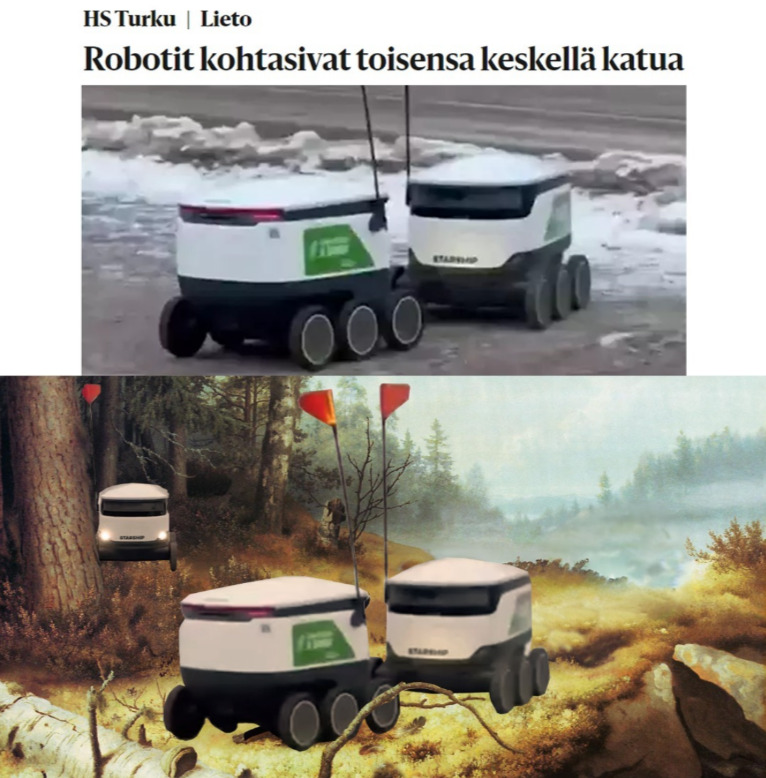
\includegraphics[width=0.95\linewidth]{assets/vainkeskiluokkajutut}
		\captionof{figure}{@vainkeskiluokkajutut:n meemi}
	\end{Figure}
	\columnbreak
	\begin{Figure}
		\vspace*{1.85cm}
		\noindent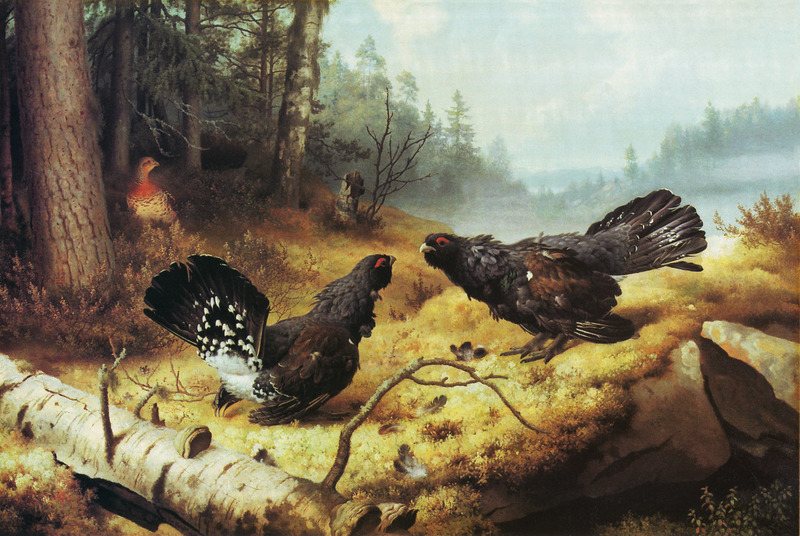
\includegraphics[width=0.95\linewidth]{assets/taistelevatmetsot}
		\captionof{figure}{Ferdinand von Wright - Taistelevat metsot}
	\end{Figure}
\end{multicols}

\vfill

Tähän kilpailuun kutsumme teidät tekemään omia remakeja kuuluisasta
suomalaisesta taiteesta. Seuraavalta sivulta löydät \textbf{esimerkiksi} muutamia maalauksia suomalaisen
taiteen kultakaudelta. Tyyli on jätetty vapaasti valittavaksi, oli se sitten
montaasi, tosielämän uudelleenversio tai mitä ikinä keksittekään.
Saatte bonuspisteitä, jos laitatte teokseenne jotain partio"-twistia!

Osallistu kilpailuun lähettämällä teoksesi Tassun päätoimittajalle sähköpostilla (osoitteen löydät lehden 
sisäkannesta) tai suoraan esimerkiksi Whatsapp"-viestillä. Muista mainita viestissäsi kaikkien teokseen 
osallistuneiden tekijöiden nimet. Julkaisemme valittuja teoksia seuraavassa Tassussa.

\clearpage
\textbf{\large Esimerkkejä:}

\begin{multicols}{2}
	\vspace*{0.30cm}
	\begin{Figure}
		\noindent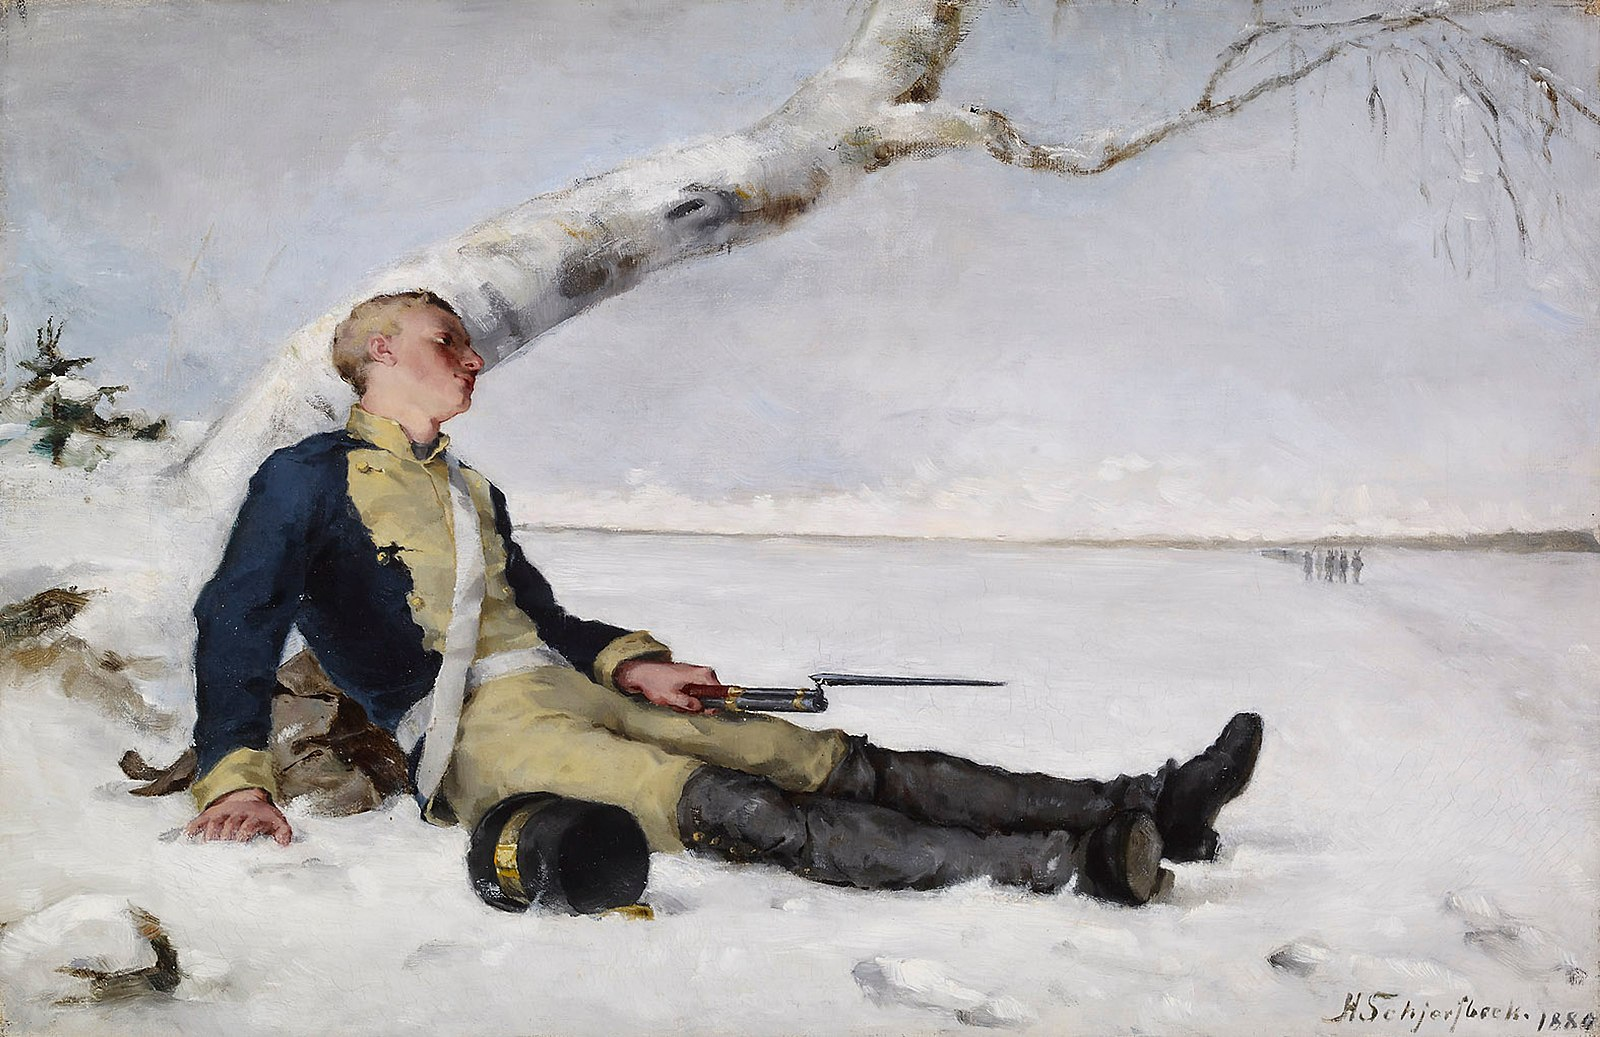
\includegraphics[width=0.95\linewidth]{assets/haavoittunutsoturihangessa}
		\captionof{figure}{Helene Schjerfbeck - Haavoittunut soturi hangessa}
	\end{Figure}
	\columnbreak
	\begin{Figure}
		\noindent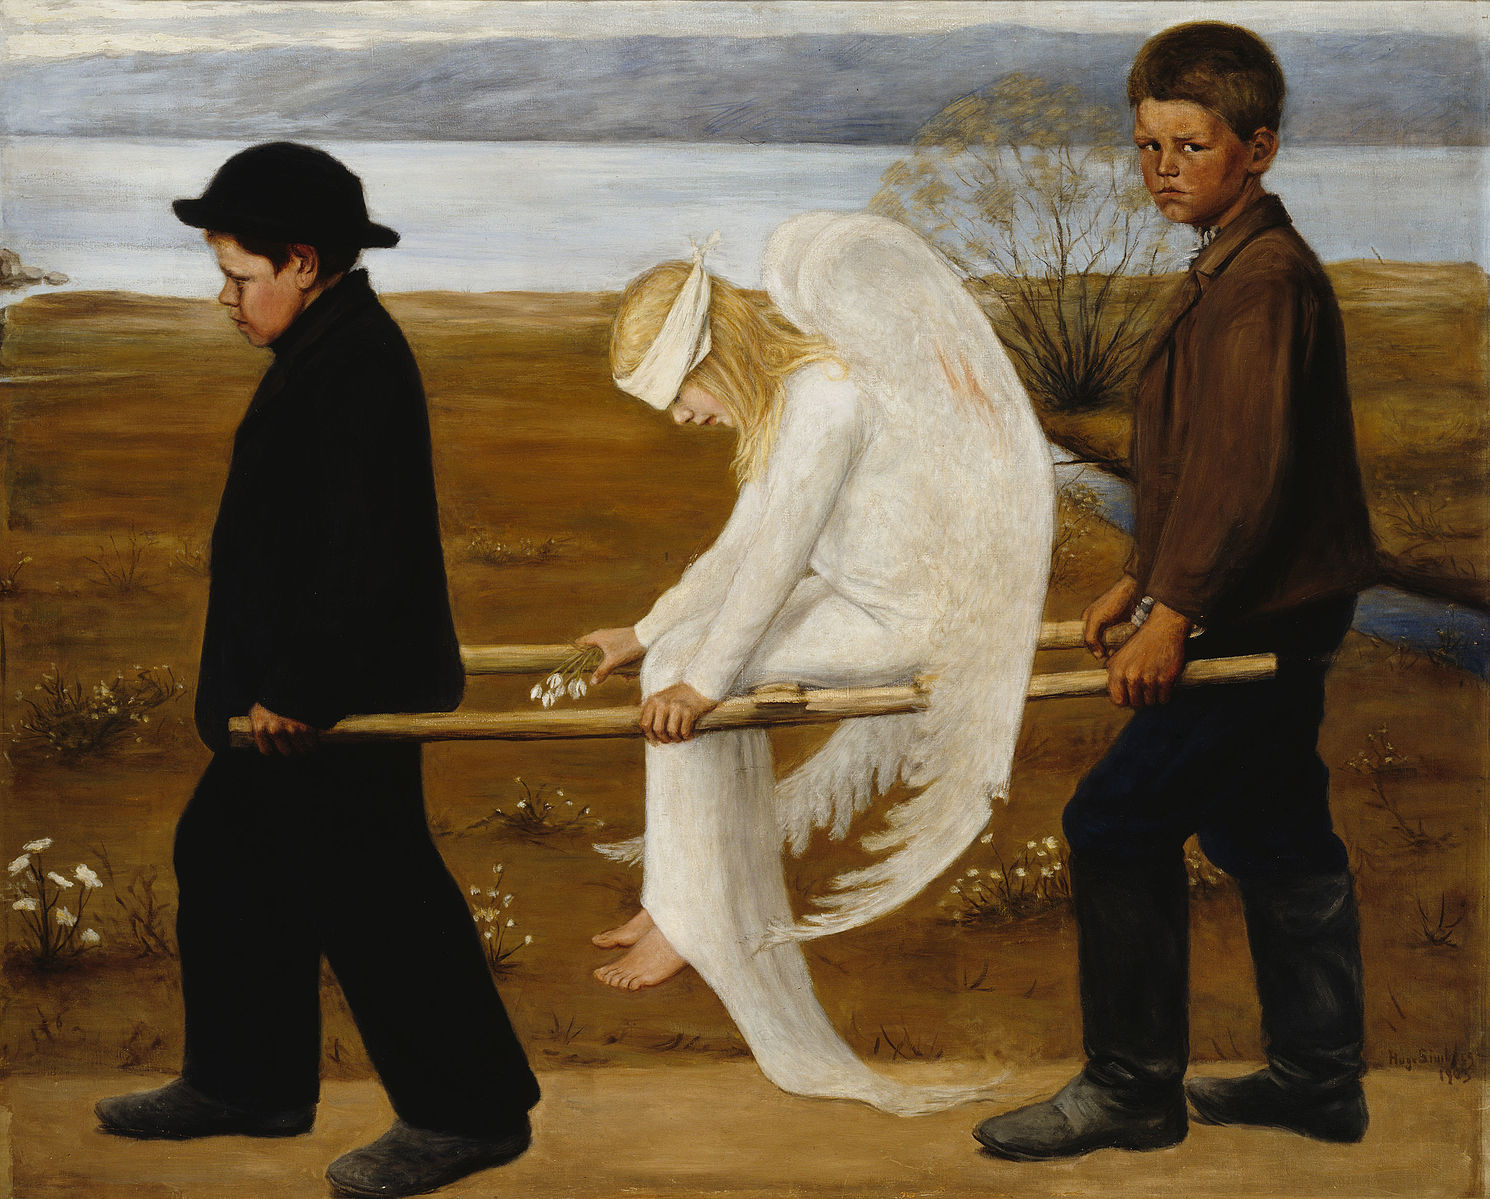
\includegraphics[width=0.95\linewidth]{assets/haavoittunutenkeli}
		\captionof{figure}{Hugo Simberg - Haavoittunut enkeli}
	\end{Figure}
\end{multicols}

\vspace*{-0.32cm}
\vspace*{-0.64cm}

\begin{multicols}{3}
	\vspace*{0.05cm}
	\begin{Figure}
		\noindent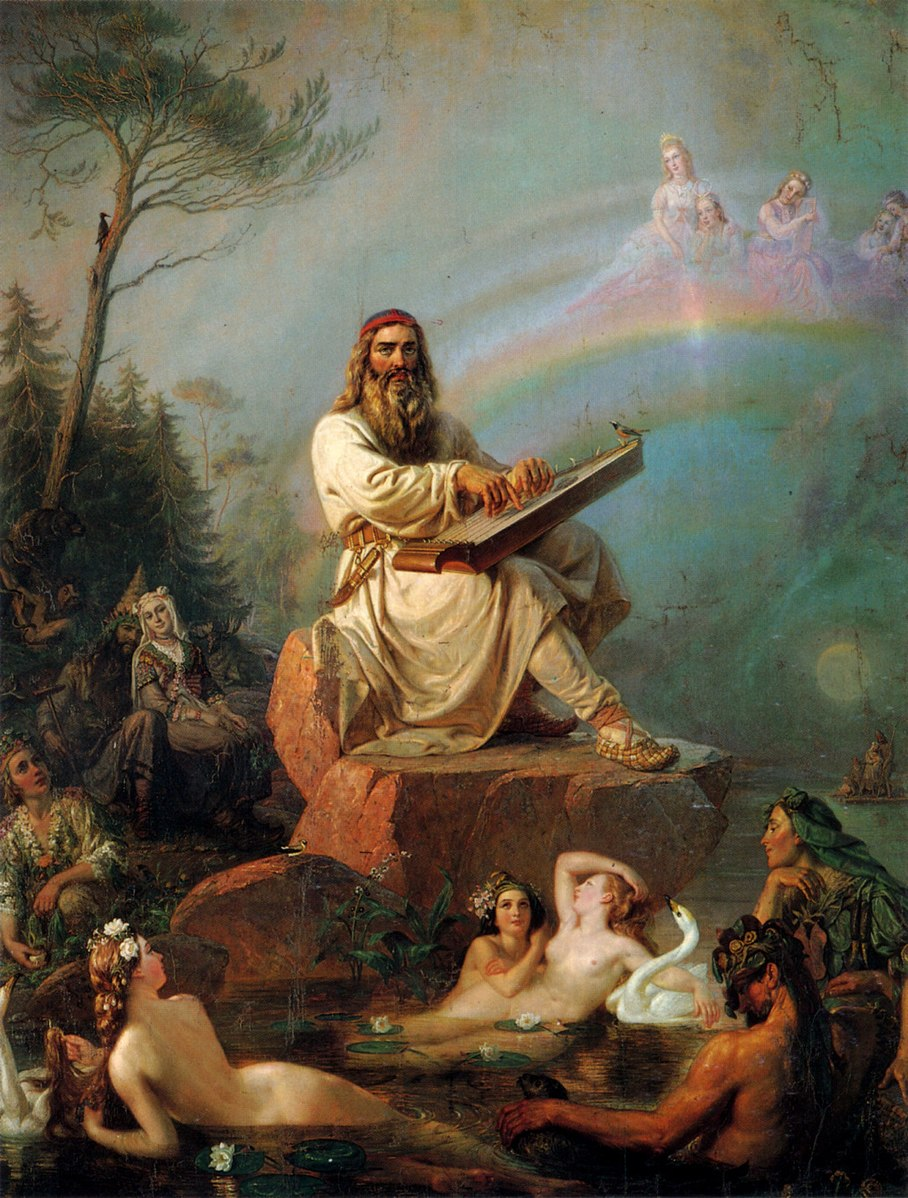
\includegraphics[width=0.90\linewidth]{assets/väinämöisensoitto.jpg}
		\captionof{figure}{Robert Wilhelm Ekman - Väinämöisen soitto}
	\end{Figure}
	\columnbreak
	\vspace*{0.05cm}
	\begin{Figure}
		\noindent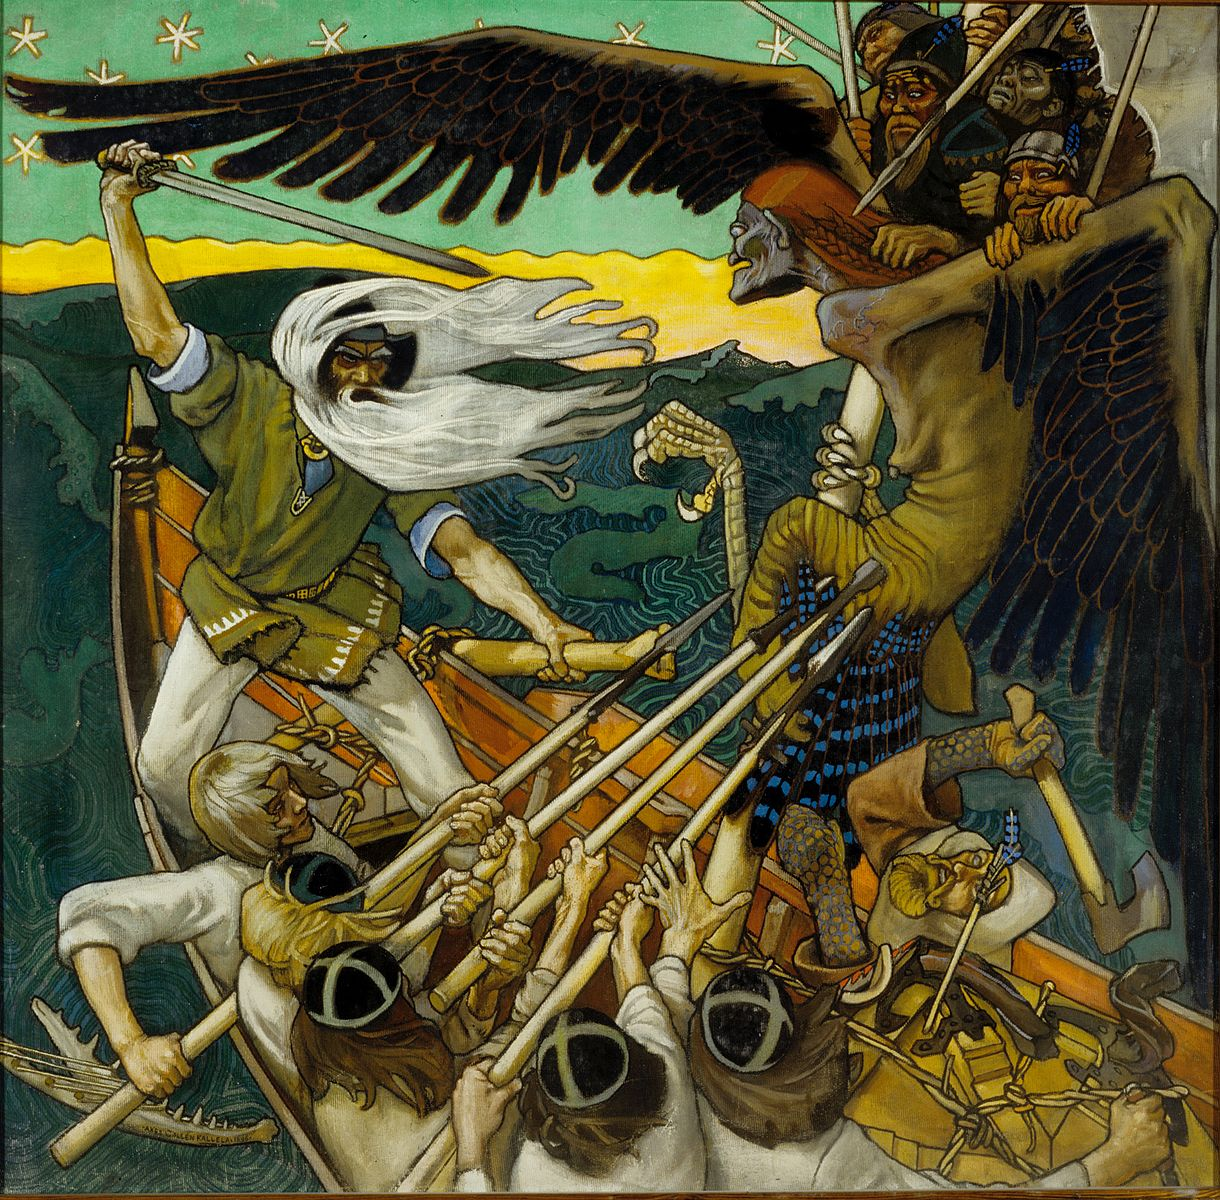
\includegraphics[width=0.90\linewidth]{assets/sammonpuolustus}
		\captionof{figure}{Akseli Gallen-Kallela - Sammon puolustus}
	\end{Figure}
	\columnbreak
	\vspace*{0.05cm}
	\begin{Figure}
		\noindent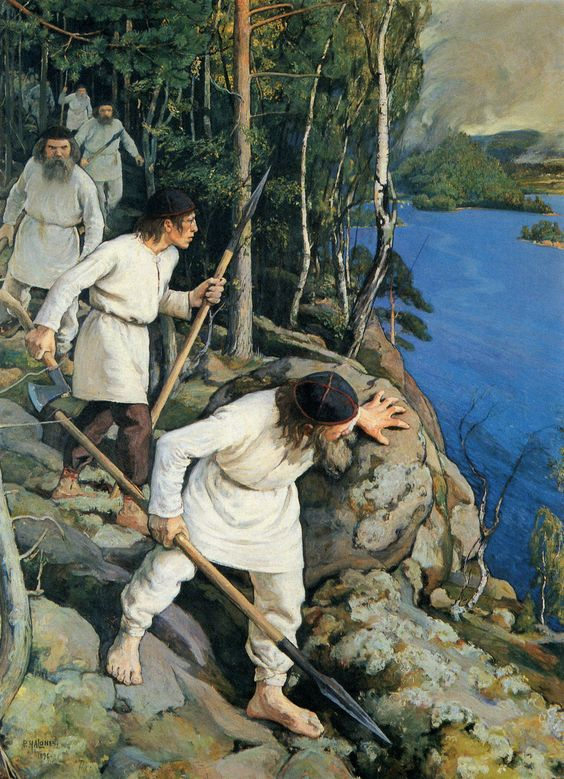
\includegraphics[width=0.90\linewidth]{assets/vainolaistavastaan}
		\captionof{figure}{Pekka Halonen - Vainolaista vastaan}
	\end{Figure}
\end{multicols}

\vspace*{0.08cm}

\begin{multicols}{2}
	\begin{Figure}
		\noindent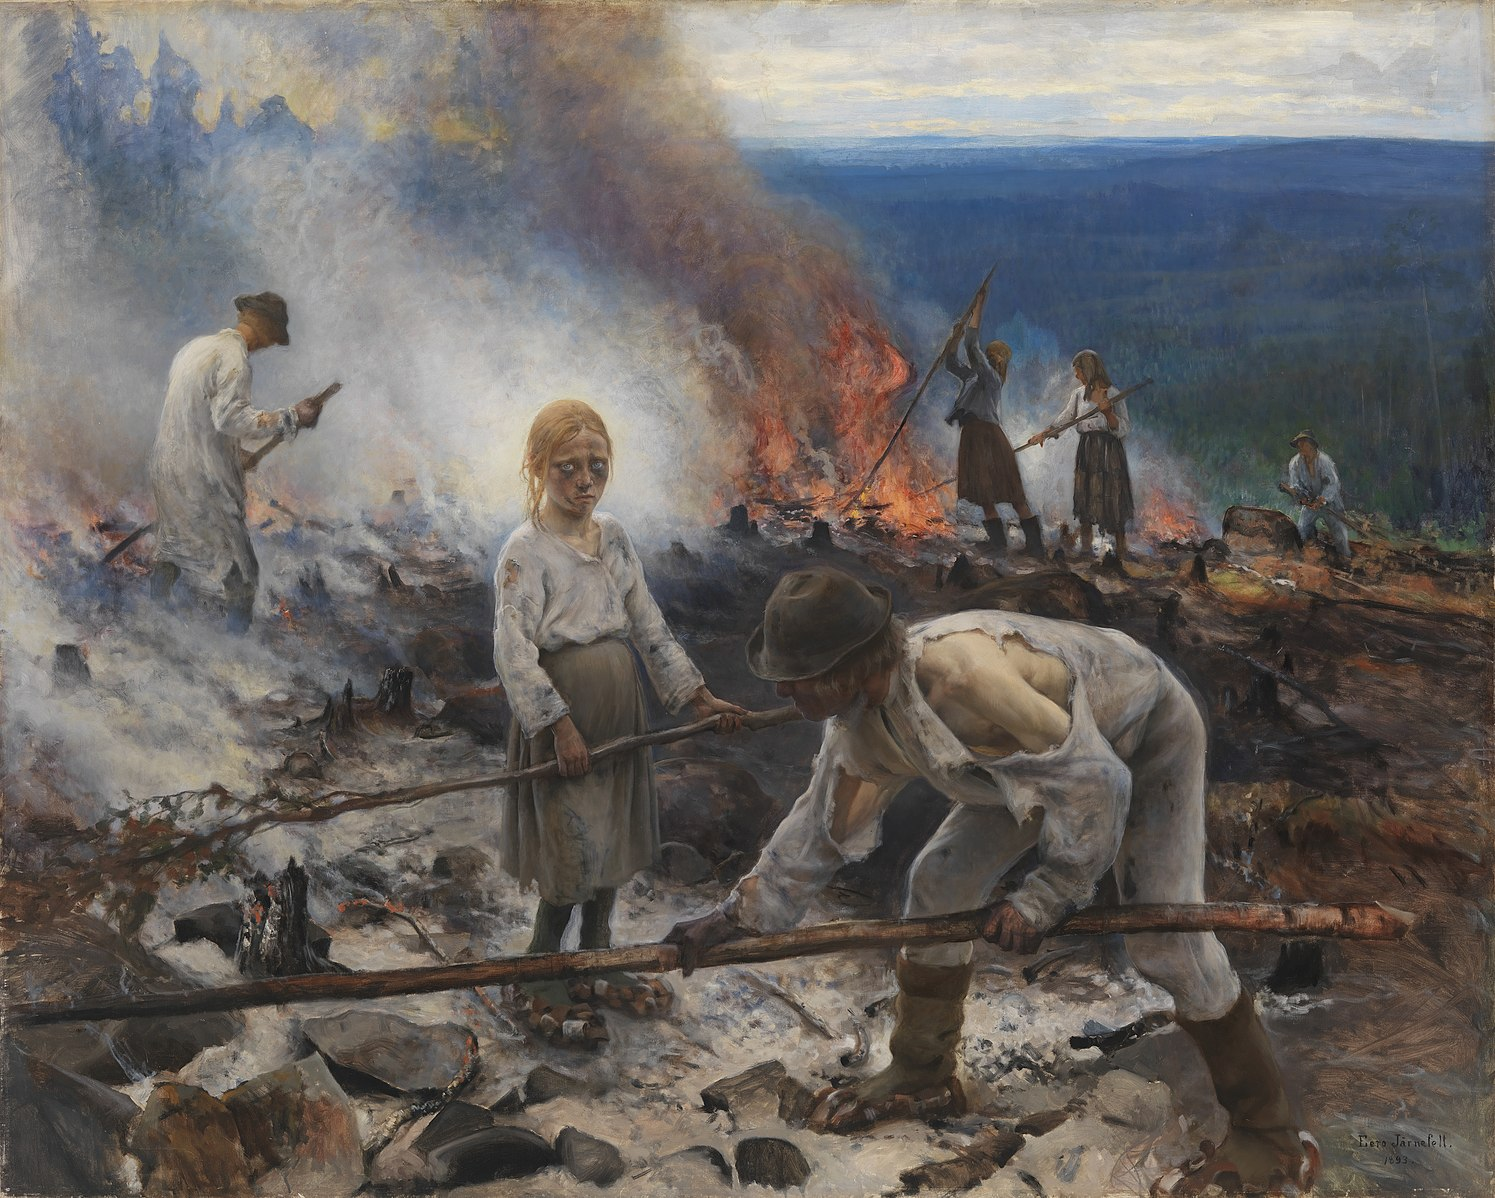
\includegraphics[width=0.95\linewidth]{assets/raatajatrahanalaiset}
		\captionof{figure}{Eero Järnefelt - Raatajat rahanalaiset}
	\end{Figure}
	\columnbreak
	\begin{Figure}
		\noindent\includegraphics[width=0.91\linewidth]{assets/leikkiviäpoikiarannalla}
		\captionof{figure}{Albert Edelfelt - Leikkiviä poikia rannalla}
	\end{Figure}
\end{multicols}
